To improve further on initialisation, this software-defined feedback loop should be shifted into an integrated solution, such as a purpose-built solution with a \gls{mcu} or \gls{fpga}. While an \gls{fpga} would be easy to apply to the problem of detecting blips and measuring time, there is a complexity in integrating an \gls{fpga} based solution with \gls{daq}. 

Data acquisition has been solely performed by a \gls{pcie} connected digitizer card, where data is dumped directly to memory and then saved to a hard-disk. If an \gls{fpga} were to be used in the manner described above, it would either need to introduce a separate \gls{daq} system, where data processed in the \gls{fpga} is collected separately from what is stored on hard-disk, or the introduced \gls{daq} would need to also store its data for analysis.

\begin{figure}[htbp]
	\centering
	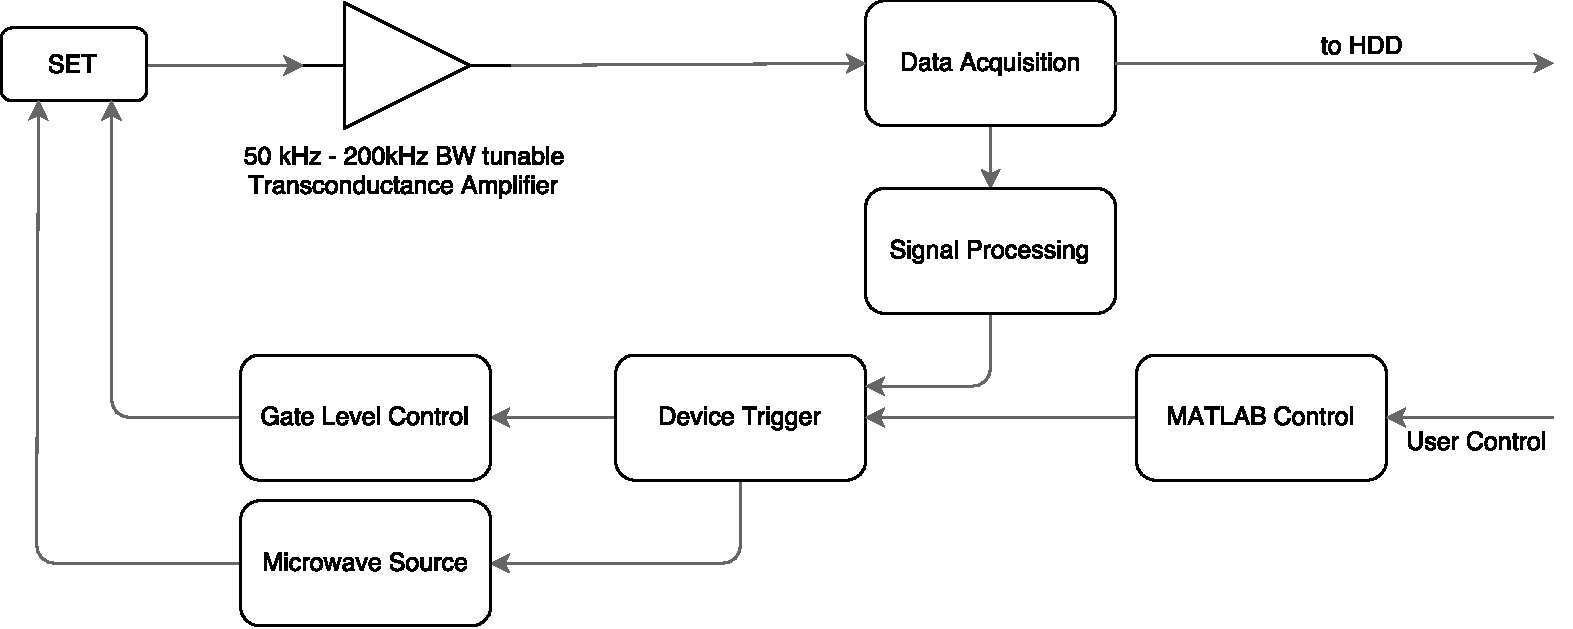
\includegraphics[width=\textwidth]{thesis_redesign_1}
	\caption{An integrated solution which writes data back to disk.}
	\label{fig::redesign_1}
\end{figure}

The first solution holds far more complexity, as it requires designing a system with a \gls{daq} and an \gls{fpga}. This would likely end up using a custom \gls{pcb}, with a special purpose \gls{adc}. The construction and verification of such a device is an undertaking not suited for a research environment where this is not the end product. Similarly, the second solution is not ideal. Storing data from an \gls{fpga} would again require specialised hardware to interface with a hard-disk. 


\begin{figure}[htbp]
	\centering
	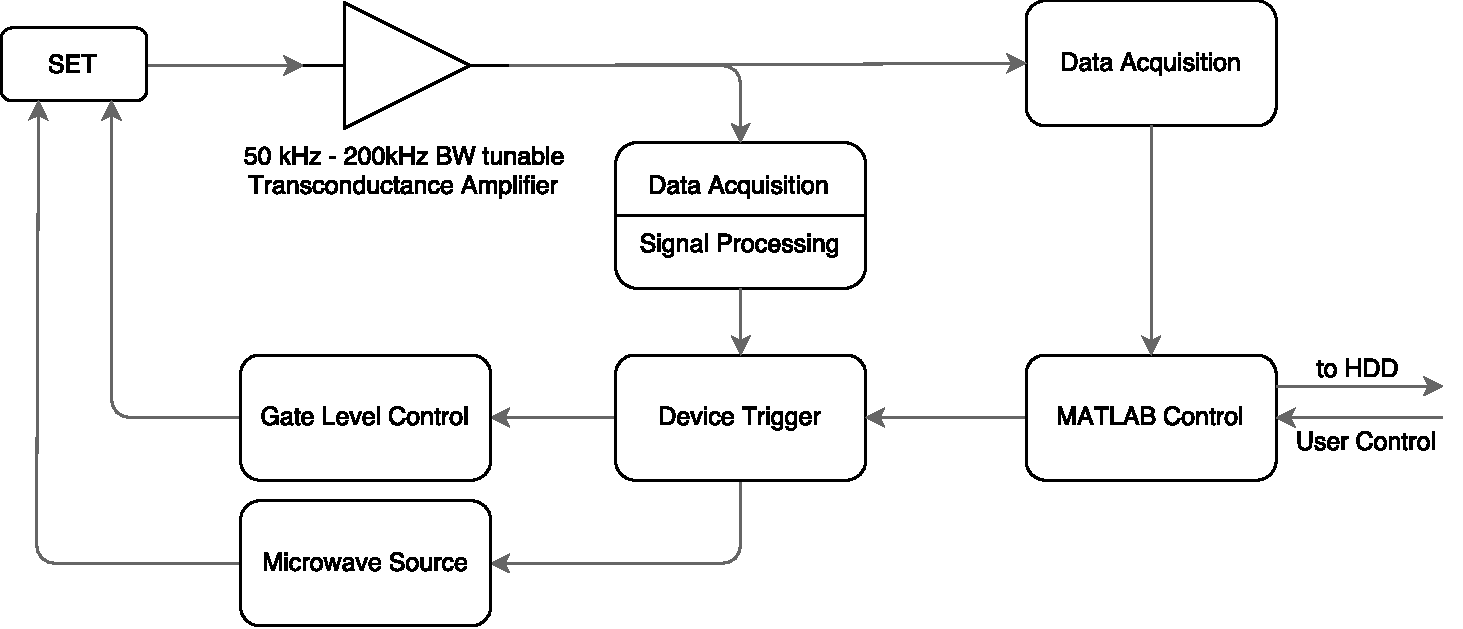
\includegraphics[width=\textwidth]{thesis_redesign_2}
	\caption{An integrated solution which adds a separate data acquisition stage to the feedback loop.}
	\label{fig::redesign_2}
\end{figure}

Ultimately, the desired solution should be integrated in a manner fit for use by non-electronic specialists. As such, a rework of the current set-up will be the preferred method of achieving real-time digital feedback.

The proposed solution is to utilise a \gls{pxie} cabinet with multiple slots to integrate the varied signals and sources we use, including an \gls{awg} and a \gls{daq}. For the problem at hand, there exist combination \gls{fpga} and \gls{daq} cards that allow for pre-processing data and controlling a single digital output, or in more advanced devices, controlling an \gls{awg} via the \gls{fpga}. This solution will be sufficient for performing threshold analysis on a single channel, however it does not make the most of the advantage an \gls{fpga} has over a \gls{mcu}. It has been shown internally in an unpublished form that a \gls{dwt} can detect blips that occur below the threshold level, due to the finite bandwidth of the device and sampling rate of the \gls{daq}.

A Haar \gls{dwt} was used in post-processing data to yield a high-fidelity readout. If this is combined with the initialisation scheme defined in this report, total experiment fidelity is expected to increase much further for lower steering times, and ultimately be more reliable. It would also allow the amplifier bandwidth to be opened up, as the increase in noise will be filtered by the transform. \gls{dwt} implementations in hardware \cite{PeiYinChen2004,hsieh2006novel,Salama2006} are commonplace, and highlight the validity and potential of an integrated \gls{fpga} based solution to the problem assessed in this thesis. 


